\section{Implementation}
The implementation of distance measurement has been done by using the method of time of flight. There are two stations each mounted with transmitter and receiver module respectively. The transmitter module contains a ultrasonic transmitter and receiver section contains a ultrasonic receiver and we measure the time of flight of the sound signal that originates from the transmitter station ending up at the receiver station.
\subsection{Transmitter Section}
The transmitter module is run with a PWM generated form a microcontroller. The overall block diagram of transmitter section is given in Figure. \ref{fig:TransmitterBlock}

\begin{figure}[h!]
	\centering
	\includegraphics[width=120mm]{Images/TransmitterBlock.png}
	\caption{Transmitter Module Block Diagram}
	\label{fig:TransmitterBlock}
\end{figure}

\subsubsection{Synchronization}
Synchronization is the most crucial part of the whole process of distance measurement. The receiver must exactly know when the transmitter is going to send the incoming signal in order to have the prior knowledge to start the time within it. It is not possible to know when exactly the transmitter will send the incoming signal but we can achieve somewhat close approximation by the use of light transmitter and receiver. 

The speed of light is approximately $3\times 10^8 m/s$. If we set up transmitter such that the transmitter station sends a pulse of light and sound at the same time, the light pulse reaches the receiver at no time compared to the sound pulse due to the massive difference of speed of each of these.

\subsubsection{Calculation}
If the distance between light transmitter and receiver is $x$, then the time taken by light to reach the receiver station is 
\begin{equation}
	t_l = \frac{x}{c}
\end{equation}
Where $t_l$ is the time taken by light to reach the receiver station. Similarly time taken by sound to reach the receiver station is given by the relation.

\begin{equation}
	t_s = \frac{x}{v_s}
\end{equation}
where $v_s$ is the speed of sound.

Now as soon as the receiver station detects the light signal, we start the timer and stop the timer as soon as it detects the sound signal.
The time recorded by the receiver station will thus be 
\begin{equation} \label{eq:deltaT}
	\Delta t = x\left( \frac{1}{v_s}- \frac{1}{c}\right)
\end{equation}
Since $c >> v_s$ $\Delta t \approx \frac{x}{v_s}$. 
The error committed in the process is 
\begin{equation} 
	\epsilon = x\left( \frac{1}{v_s}- \frac{1}{c}\right) - \frac{x}{v_s}
\end{equation}

Which gives us the error percentage of 
\begin{eqnarray*}
	Error \% & =& \frac{\epsilon}{t_s}\times 100\%\\
	{}& = & \frac{v_s}{c} \times 100 \%\\
	{}& \approx & 0.0001\% 
\end{eqnarray*}

We thus place at the transmitter side a \gls{irled} and a ultrasonic signal transmitter. At the receiver we place ultrasonic receiver and a TSOP. The TSOP detects the light signal.

\begin{figure}
	\centering
	\includegraphics[width=120mm]{Images/DetectionByTSOP.jpg}
	\caption{TSOP response to detected IR signal by IRLED}
	\label{fig:DetectionByTSOP}
\end{figure} 
In Figure.\ref{fig:DetectionByTSOP} the upper waveform is the signal fed to the \gls{irled} transmitter and the lower waveform is the response of TSOP circuitory to the detected signal.

\subsubsection{Ultrasound Transmission}
The ultrasonic transmitter typically works at a frequency of $40kHz$. So we generate the required signal using  a microcontroller. The microcontroller generates the required signal by pulling a particular pin at high and low at calculated intervals. Following piece of code is written in C for ATmega8 to generate 40kHz signal at a particular pin.

\begin{lstlisting}
void DriveIRLED()
{
	int Peaks = 5;
	int i = 0;
	for(;i< Peaks*2; i++) {
		TOGGLE(PORTC,PC5);
		_delay_us(12);
	}
}
\end{lstlisting}

\begin{figure}
	\centering
	\includegraphics[width=120mm]{Images/UltrasonicTransception.jpg}
	\caption{Signal Transmission and Reception by Ultrasonic pair}
	\label{fig:UltrasonicTransception}
\end{figure}
In Figure.\ref{fig:UltrasonicTransception} the lower signal with regular spikes is the signal applied to Ultrasonic transmitter. Each spike (contracted in time) is a brust of square wave pulses shown in Figure.\ref{fig:SignalBrust}. The interval of each burst is $2ms$. The upper signal in Figure.\ref{fig:UltrasonicTransception} is the response of Ultrasonic receiver to the obtained signal. There are clear spikes  detected at exactly the interval sent by the transmitter.
\begin{figure}
	\centering
	\includegraphics[width=120mm]{Images/SignalBrust.jpg}
	\caption{40kHz Signal Brust applied at ultrasonic transmitter}
	\label{fig:SignalBrust}
\end{figure}
 
Since the received signal is noisy and very low power, it requires to be amplified and 
filtered for the required frequency.
\subsection{Receiver Section}
The reciever section is collects thre signal transmitted by the transmitter module. The overall block diagram of the receiver module is given in Figure. \ref{fig:ReceiverOne}
\begin{figure}[h!]
	\centering
	\includegraphics[width=120mm]{Images/ReceiverOne.png}
	\caption{Receiver Module Block Diagram}
	\label{fig:ReceiverOne}
\end{figure}

\subsubsection{Signal Amplification}

The received sound signal is converted into electrical signal by ultrasonic receiver. Since the sound undergoes massive attenuation in air, the received signal is pretty low in voltage and needs to be amplified in order to use it for distance measurement. 

An amplifier is an electronic device that increases the power of a signal. An operational amplifier ("op-amp") is a DC-coupled high-gain electronic voltage amplifier with a differential input and, usually, a single-ended output. In the configuration as shown in \ref{fig:InvertingAmplifier}, an op-amp produces a output potential that is typically hundreds of thousands of times larger than the potential difference between its input terminals. 

\begin{figure}[h]
	\centering
	\begin{circuitikz}[scale=0.75,transform shape] \draw
		(4,-.5) node[op amp](opamp1) {}
		
		(1,0) node[anchor=east] {$V_{in}$}	
		to [R=$R_g$,o-*] (opamp1.-)
		to [short](2.8,1)
		to [R=$R_f$] (5.2,1)
		to [short,-*] (opamp1.out)
		
		(opamp1.out) to [short,-o] (6.2,-0.5)
		node[anchor=west] {$V_{out}$}
		(opamp1.+) to [short] ($(opamp1.+)+(0,-1)$)node [ground] {}
		;
		
	\end{circuitikz}
	\caption{A negative feedback inverting Amplifier}
	\label{fig:InvertingAmplifier}
\end{figure}


The output voltage of this operational amplifier closed loop negative feedback is given by :-
\begin{equation}
	V_{out} = -\frac{R_f}{Rg}V_{in}
\end{equation} 


Where,\\ $R_f$ is feedback resistor \\$R_g$ is input resistance. \\$V_{in}$ is input voltage, \\$V_{out}$ is output voltage. 

The gain of the amplifier is controlled by two resistors, $R_f$ and $R_g$. The gain is the ratio of the feedback resistor to the input resistor. However, the opamp we used,i.e. IL741 has a maximum practical gain of 2.5 dB only. Since the electrical signal produced by the ultrasonic receiver is pretty low in voltage, it needs to be amplified with amplifier having very high gain. This task of amplifying the received pretty low voltage signal is carried out by an instrumentation amplifier. The circuit diagram for instrumentation amplifer is as shown in \ref{fig:InstrumentationAmplifier}

\subsubsection{Instrumentation Amplifier}
The main disadvantages of the differential amplifier or single operational amplifier are its low input impedances and low common mode rejection ratio \gls{cmrr}.  Such kind of problems can be solved by using instrumentation amplifier. Instrumentation amplifier is a high precision amplifier with an adjustable gain having high \gls{cmrr} and input impedance. It is a kind of differential amplifier with additional input buffers. It uses 3 operational amplifiers, the first two amplifier acts as the buffer which has very high input impedance and low output impedance and the latter one is used as a differential amplifier to amplify the signal applied to its input. The advantage of the input buffers stages makes it easy to match the impedance of the amplifier with the preceding stage. The inputs are applied to the first two operational amplifiers. The difference in the applied signal is only amplified by the amplifier but it rejects the common signal applied to its inputs. So whatever the environment is, the noise signal gets rejected. Its output impedance is very low so that there is low signal attenuation to transfer the whole amplified signal to the required circuit. Instrumentation amplifier is used for the higher accuracy and the stability of the circuit.

\begin{figure}[h]
	\centering
	\begin{circuitikz}[scale=0.7,transform shape] \draw
		(4,4.5) node[op amp,,yscale=-1](opamp1) {}
		(4,-2.5) node[op amp](opamp2) {}
		(10,1) node[op amp](opamp3) {}
		(1,5) node[anchor=east] {$V_1$}	
		to [short,o-] (opamp1.+)
		(1,-3) node[anchor=east] {$V_2$}	
		to [short,o-] (opamp2.+)
		(opamp1.out) to [R=$R_1$,*-*] ($(opamp1.out)+(0,-2)$)
		to [R=$R_{gain}$,*-*] ($(opamp1.out)+(0,-5)$)
		to [R=$R_1$,*-*] (opamp2.out)
		($(opamp1.out)+(0,-2)$) to [short] ($(opamp1.-)+(0,-1.5)$)
		to [short] (opamp1.-)
		($(opamp1.out)+(0,-5)$) to [short] ($(opamp2.-)+(0,1.5)$)
		to [short] (opamp2.-)
		(opamp1.out) to [R=$R_2$,*-*] ($(opamp3.-)+(0,3)$)
		to [short] (opamp3.-)
		(opamp2.out) to [R=$R_2$,*-*] ($(opamp3.+)+(0,-3)$)
		to [short] (opamp3.+)
		($(opamp3.-)+(0,3)$) to [R=$R_3$,*-] ($(opamp3.out)+(0,3.5)$)
		to [short] (opamp3.out)
		($(opamp3.+)+(0,-3)$) to [R=$R_3$,*-] ($(opamp3.out)+(0,-3.5)$)
		node[ground] {}
		(opamp3.out) to [short,*-o] ($(opamp3.out)+(2,0)$)
		node[right] {$V_3$}
		;
		
	\end{circuitikz}
	\caption{Instrumentation Amplifier}
	\label{fig:InstrumentationAmplifier}
\end{figure}


The gain of the instrumentation amplifier is given as:
\begin{equation}
	\frac{V_{out}}{V_1-V_2}=(1+\frac{2R_1}{R_{gain}})\frac{R_3}{R_2}
\end{equation}
where, $V_1$ and $V_2$ are the signals applied to the non-inverting inputs of operational amplifiers. The gain of the amplifier can be adjusted by changing the resistor value $R_{gain}$. We have used a potentiometer in place of the $R_gain$ so that the value of the gain can be adjusted. For the simplification other resistor values are kept same. 

Similarly, the \gls{cmrr} of the instrumentation amplifier can be written in terms of \gls{cmrr} of the single operational amplifier as:
\begin{equation}
	CMRR_{ins-amp}=(1+2\frac{R_1}{R_gain})CMRR_{op-amp} \nonumber
\end{equation}
Hence the \gls{cmrr} of the intrumentation amplifier is $(1+2\frac{R_1}{R_{gain}})$ times greater than that of a single operational amplifier.

	
Thus the low voltage signal received through the receiver of ultrasonic sensor is amplified using instrumentation amplifier circuit. The values of the component of this operational amplifier is calculated so that the required signal strength can be achieved. The amplified signal is now fed into the input of tone decoder circuit.


\subsubsection{Signal Filtering}

The transducer will pick up most sounds within a fairly wide range. Thus ultrasonic signal received by the receiver not just contain the 40kHz required signal. It also comprises of some other noise signals. To make sure the system only picks up the ultrasound signal that was transmitted, we need to lock the receiver onto a frequency of 40kHz. 

For this, we have used IL567 Tone Decoder \gls{ic}. This tone decoder is a general purpose tone decoder which looks for a close match between the frequency of incoming signal and of its internal oscillator. The frequency of it's internal oscillator can be controlled by adjusting the values of capacitor and resistor between Pin 5 and Pin 6 of the \gls{ic}. The frequency of internal oscillator is given by the expression :\cite{Yichao}

\begin{equation}
	f=\frac{1}{1.1*R*C}
\end{equation}
where,
R = Resistor placed between Pin 5 and Pin 6
C = capacitor placed at Pin 6
\begin{figure}[h]
	\centering
	\includegraphics[scale=0.5]{Images/IL567PinOut.jpg}
	\caption{IL567 Pin Out}
	\label{fig:PinOut}
\end{figure}

\begin{table}[h!]
	\centering
	\caption{Pin Description of IL567 \gls{ic}\cite{ToneDecoder}}
	\begin{tabular}{|c|c|c|}
		\hline 
		\bf{Pin Number} & \bf{Symbol} & \bf{Description} \\ 
		\hline 
		01 & OF & FIlter output \\	
		02 & LF & Loop Filter \\
		03 & IN & Frequency Input \\	  
		04 & $U_{cc}$ & Supply Voltage \\	  
		05 & TR & Timing Resistor \\	  
		06 & TC & Timing Capacitor \\	  
		07 & GND & Common Pin(Ground) \\	  
		08 & OUT & Output \\ 
		\hline 
	\end{tabular} 
\end{table}

This IC sets it's output(Pin 8) to low when the frequency of incoming signal matches the frequency of internal oscillator. When there is incoming signal of other frequencies or there is no signal at all, the output(Pin 8) remains high. 
We used a capacitor of 0.01$\mu$ F. In order to lock the frequency of internal oscillator at 40kHz, we need a resistor of approximately 2.272 K$\Omega$ . Now since exactly this value resistor was not available, we used a potentiometer of 10K instead of this resistor. 

\subsubsection{Fixing the frequency of internal oscillator}

To make sure that the tone decoder recognizes 40kHz signal and sets it output to low only on the arrival of 40kHz signal, the frequency of it's internal oscillator needs to be fixed at 40kHz. Since we do not have exactly 2.272K$\Omega$ resistor available, we use a potentiometer to adjust the frequency of internal oscillator.

We fed a 40kHz sinusoidal signal to the input of the IL567 from function generator. Since the output of the IC is high when the frequency of incoming signal does not match the frequency of internal oscillator or also when there is no signal whatsoever, initially the output of this IC was high. Now the potentiometer was adjusted until the output of the IC was low. Thus, the frequency of internal oscillator of the IL567 was finalised to 40kHz.
\begin{figure}[h]
	\centering
	\includegraphics[scale=0.7]{Images/ToneDecoder.jpg}
	\caption{Circuit Diagram for Tone Decoding}
	\label{fig:CircuitDiagramForToneDecoding}
\end{figure}

\subsubsection{Detection of Incoming Signal}
The ultrasonic receiver receives the 40kHz signal transmitted from the transmitter. This signal is amplified using a two stage operational amplifier. The output of the amplifier circuit is fed as an input to the IL567. Now, as soon as the output of the IL567 goes low, we can know that the incoming signal is the transmitted signal with frequency of 40kHz. Thus, this can operate as a bandpass filter at 40kHz.

The output pin (Pin 8) on the LM567 Tone Decoder is connected to an input configured I/O pin on the microcontroller so that it is able to detect signals from the LM567 Tone Decoder. When the output pin (Pin 8) on the LM567 Tone Decoder is pulled low, the microcontroller knows that an ultrasonic signal has been received, and it stops running the counter and calculates the travel time of the signal.

\subsection{Distance Calculation}
Now equipped with all these stages we are finally able to calculate the distance between the transmitter and receiver station. Since we have the time recorded, we can use the time recorded using Equation.\ref{eq:deltaT} to calculate the original distance. Let the time recorded by the receiver station be $T_r$. Then we can use this recorded time to calculate distance as
\begin{eqnarray*}
	d &=& T_r \times v_s\\
	{}&=&\Delta t \times v_s\\
	{}&\approx&\frac{x}{v_s} \times v_s\\
	{}& = & x
\end{eqnarray*}
Thus we can find the actual distance $x$ by this process.

\subsection{Data Collection}
The distance measured by this process is collected in each of the three receiver station. The data collected in each of the three receiver station should be collected in one microcontroller to transmit to the computer.  The overall block diagram of the data collection section is given in Figure. \ref{fig:MasterSlave}

\begin{figure}[h!]
	\centering
	\includegraphics[width=120mm]{Images/MasterSlave.png}
	\caption{Data Collection Section Block Diagram}
	\label{fig:MasterSlave}
\end{figure}


\subsubsection{Communication Between Microcontrollers}
The output of tone decoder is either a logic high or a logic low. Logic high means the receiver is not receiving the required signal and logic low means that receiver is receiving required transmitted $40kHz$ ultrasonic signal.

The output of the tone decoder is fed into one of the $I/O$ pin of microcontroller ATMega8. Similarly, we have output of TSOP fed into another pin of the same microcontroller. The difference between time of arrival of the infrared signal, which is denoted by the output of TSOP and that of ultrasonic signal, which is denoted by the output of tone decoder is used for finding the distance between transmitter and receiver. All the calculations are performed within the microcontroller and thus the microcontroller contains the information of distance between transmitter and receiver.

In this way, all three microcontrollers residing on receiving modules comprise the information of distance between respective transmitters and receivers. All these distances are essential to determine the location of the transmitter using trilateration. As explained on the methodology section, when the distances between the transmitter and three predefined receivers are known, the location of a transmitter can be determined using trilateration.

This task of communicating between the microcontrollers is achieved by using \gls{spi}. \gls{spi} is one of the most used serial communication protocols.The \gls{spi} allows high-speed synchronous data transfer between the AVR and peripheral devices or between several AVR devices. The interconnection between two \gls{spi} devices always happens between a master device and a slave device. Compared to some peripheral devices like sensors which can only run in slave mode, the \gls{spi} of the AVR can be configured for both master and slave mode. The mode the AVR is running in is specified by the settings of the master bit (MSTR) in the \gls{spi} control register (SPCR). Special considerations about the SS pin have to be taken into account. This will be described later in the section “Multi Slave Systems - SS pin Functionality on page 3. The master is the active part in this system and has to provide the clock signal a serial data transmission is based on. The slave is not capable of generating the clock signal and thus can not get active on its own. The slave just sends and receives data if the master generates the necessary clock signal. The master however generates the clock signal only while sending data. That means that the master has to send data to the slave to read data from the slave.

\subsubsection{Data Transmission Between Master and Slave}
The interaction between a master and a slave AVR is shown in Figure \ref{fig:Interaction}. Two identical SPI units are displayed. The left unit is configured as master while the right unit is configured as slave. The MISO, MOSI and SCK lines are connected with the corresponding lines of the other part. The mode in which a part is running determines if they are input or output signal lines. Because a bit is shifted from the master to the slave and from the slave to the master simultaneously in one clock cycle both 8-bit shift registers can be considered as one 16-bit circular shift register. This means that after eight SCK clock pulses the data between master and slave will be exchanged.
\begin{figure}[htpb]
	\centering
	\includegraphics[scale=0.85]{Images/MasterandSlave.png}
	\caption{Interaction between a master and a slave}
	\label{fig:Interaction}
\end{figure}

The system is single buffered in the transmit direction and double buffered in the receive direction. This influences the data handling in the following ways:

\begin{enumerate}
	\item New bytes to be sent can not be written to the data register (SPDR) / shift register before the entire shift cycle is completed.
	\item Received bytes are written to the Receive Buffer immediately after the transmission is completed.
	\item The Receive Buffer has to be read before the next transmission is completed or data will be lost.
	\item Reading the SPDR will return the data of the Receive Buffer.
\end{enumerate}

After a transfer is completed the SPI Interrupt Flag (SPIF) will be set in the SPI Status Register (SPSR). This will cause the corresponding interrupt to be executed if this interrupt and the global interrupts are enabled. Setting the SPI Interrupt Enable (SPIE) bit in the SPCR enables the interrupt of the SPI while setting the I bit in the SREG enables the global interrupts.

\subsubsection{SPI Pins}
The SPI consists of four different signal lines. These lines are the shift clock (SCK), the Master Out Slave In line (MOSI), the Master In Slave Out line (MISO) and the active low Slave Select 3 line (SS). When the SPI is enabled, the data direction of the MOSI, MISO, SCK and SS pins are overridden according to the table.
\begin{table}[htpb]
\centering
\caption{SPI pin overrides}
\label{tab:Pinoverrides}
\begin{tabular}{|c|c|c|}
\hline 
Pin & Direction Master Mode & Direction Slave Mode \\ 
\hline 
MOSI & User Defined & Input \\ 
\hline 
MISO & Input & User Defined \\ 
\hline 
SCk & User Defined & Input \\ 
\hline 
$\overline{SS}$ & User Defined & Input \\ 
\hline 
\end{tabular} 
\end{table}

\subsubsection{Multi-Slave System}
The Slave Select $\overline{SS}$ pin plays a central role in the SPI configuration. Depending on the mode the part is running in and the configuration of this pin, it can be used to activate or deactivate the devices. The $\overline{SS}$ pin can be compared with a chip select pin which has some extra features. In master mode, the $\overline{SS}$ pin must be held high to ensure master SPI operation if this pin is configured as an input pin. A low level will switch the SPI into slave mode.

The ability to connect several devices to the same SPI-bus is based on the fact that only one master and only one slave is active at the same time. The multi-slave system is demonstrated by Figure \ref{fig:Multislave}.

\begin{figure}[htpb]
	\centering
	\includegraphics[scale=1]{Images/Multislave.png}
	\caption{Multi-Slave System}
	\label{fig:Multislave}
\end{figure}
Thus, the slave select pin of the slave whose data is to be transmitted to the master is held low at a time while the slave select pins of other slaves are held high. Thus, the master also knows from which slave it is receiving the data.

Thus, all three distances need to be fed into one another computational device for determining the location of the transmitter. Thus, all three microcontrollers send the information of distance into one another microcontroller, which feeds the data to PC via \gls{usb} cable where the task of locating the transmitter is done.



\subsection{Communication between Microcontroller and PC}
 V-USB is a very useful software-only implementation of low-speed USB device for AVR microcontrollers. It adds USB functionality for almost any AVR, particularly for those without hardware USB functionality. The communication with PC has two distinct parts:
\begin{enumerate}
	\item Firmware on Device
	\item Host Driver Software on PC
\end{enumerate}

\subsubsection{Firmware}
To make the interface to communicate with pc we have used VUSB library. This library helps to communicate data between PC and the microcontroller. The firmware does the necessary tasks required for preparation of putting the data in device buffer and send data to the PC following the \gls{usb} protocol. These data is sent to the PC through \gls{usb} cable.


\subsubsection{Host Software}
Once the data is received in the computer, the task remaining is to trace out the values on PC screen. For plotting this data into the screen as a function of time, we have prepared a graph plotting software ourselves, which plots the values received at the PC through \gls{usb} port into the display of the PC making the waveform of the input signals visible. 

Host software again makes use of lib \gls{usb} library to make proper communication with the firmware on the device. A channel is formed between the host software and device through the \gls{usb} connection.


The software interfaces are made in C++ programming language and compiled for Linux Operating system. But the programs are made platform independent and can be easily compiled for other operating systems with just minor changes.


\subsection{Circuit Realization}
We have made the transmitter circuit which comprises of a \gls{pwm}Generator to transmit $40kHz$ ultrasonic signal as well as a $38kHz$ \gls{ir} signal.

\begin{figure}
	\centering
	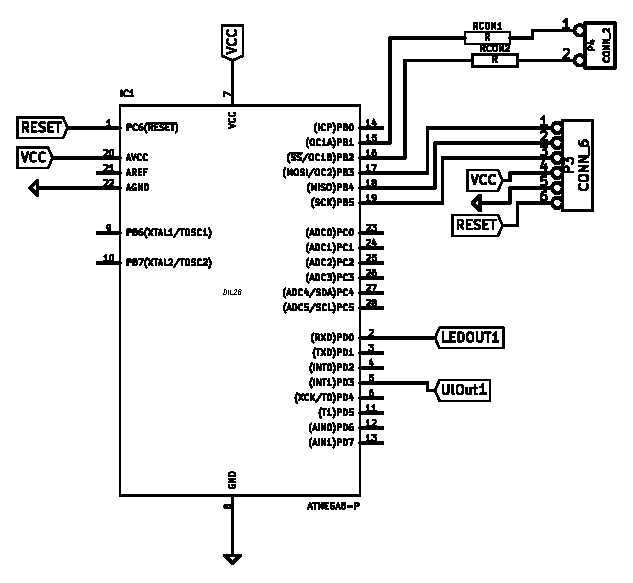
\includegraphics{Images/PWMGenerator.eps}
	\caption{PWM Signal Generator}
	\label{fig:PWMGenerator}
\end{figure}

The generated \gls{pwm} signal is fed to the Ultrasonic Transmitter, but signal sinking causes the signal to die out in the ultrasonic transmitter. So we have used a transistor to decouple the circuit from the ultrasonic transmitter. Figure.\ref{fig:Transmitter} shows the Ultrasonic transmitter attached to the output pin of \gls{pwm} generator in Atmega8.
\begin{figure}
	\centering
	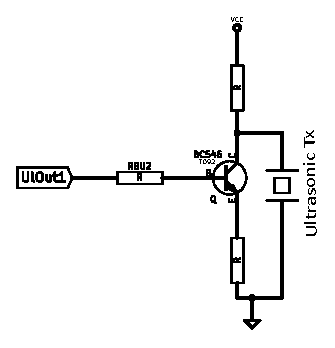
\includegraphics{Images/Transmitter.eps}
	\caption{Ultrasonic transmitter driven by \gls{pwm}}
	\label{fig:Transmitter}
\end{figure}

Also for synchronization process \gls{irled} is also driven by the microcontroller. Figure.\ref{fig:IRLEDCircuit} shows the \gls{irled} attached to the \gls{pwm} generator.

\begin{figure}
	\centering
	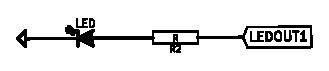
\includegraphics{Images/IRLEDCircuit.eps}
	\caption{\gls{irled} driven by \gls{pwm}}
	\label{fig:IRLEDCircuit}
\end{figure}

Finally a \gls{pcb} is made for the transmitter which is shown in Figure.\ref{fig:TransmitterPCB}.

\begin{figure}
	\centering
	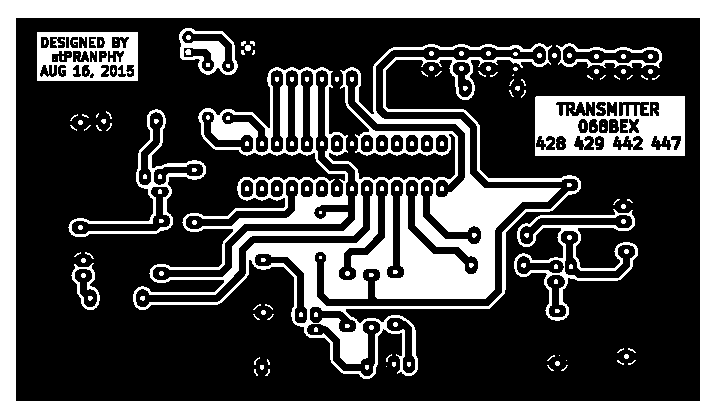
\includegraphics{Images/TransmitterPCB.eps}
	\caption{\gls{pcb} of the transmitter section}
	\label{fig:TransmitterPCB}
\end{figure}

Similarly, there are three receivers which receive the signals transmitted from transmitter section in all three directions. \gls{pcb} for the receiver is shown in Figure.\ref{fig:ReceiverPCB}
\begin{figure}[htpb]
	\centering
	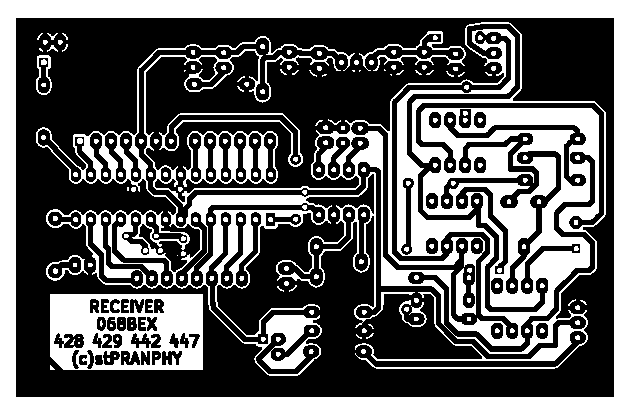
\includegraphics[scale=1]{Images/ReceiverModulePCB.eps}
	\caption{\gls{pcb} of the Receiver Module}
	\label{fig:ReceiverPCB}
\end{figure}

The receiver modules act as slave to transmit the distances to another microcontroller, which acts as a master. The implementation of master's module is as shown in Figure.\ref{fig:MasterModule}
\begin{figure}[htpb]
	\centering
	\includegraphics[scale=0.25]{Images/MasterModule.png}
	\caption{3-D view of Master Module}
	\label{fig:MasterModule}
\end{figure}
